%!TEX root = ../../../main.tex

\subsection{Evaluation}

Finally, after running a tuning session, we must treat and analyse the obtained data, in order to obtain valuable insight into the \acrshort{pca} process. To do this, we must first know what data we can process, how to present it in a graphical way and how to use the generated graphs to obtain insights.

\subsubsection{Results}

All the obtained data is handled by the Weight and Biases service, where we can evaluate each trial individually, looking into it's results and corresponding metadata. An example of what data is available for a single trial can be seen in figure \ref{tab:datapoints}

\begin{table}[ht]
\centering
\begin{tabular}{l|l}
Parameters                 & Values                 \\ \hline
config/max\_iterations     & 2456                   \\
config/sample\_size        & 562                    \\
percentage\_diff           & -0.07015456937412218   \\
timesteps\_since\_restore  & 0                      \\
\_step                     & 23                     \\
timestamp                  & 1623285355             \\
\_timestamp                & 1623285355             \\
time\_total\_s             & 2399.8914699554443     \\
iterations\_since\_restore & 18                     \\
\_runtime                  & 12445                  \\
time\_this\_iter\_s        & 47.57563805580139      \\
time\_since\_restore       & 1908.3043472766876     \\
training\_iteration        & 24                     \\
run\_time                  & 47.512633085250854     \\
max\_delta                 & -0.0005431512206575118 \\
mean\_delta                & -0.0001985753873656737 \\
avg\_percentage\_diff      & 202.68418773177495    
\end{tabular}
\caption{Data obtained from a trial through Weight and Biases}
\label{tab:datapoints}
\end{table}

Manually sifting through each trials data is a time intensive task, as a single training session can have over 100 trials and thousands of data points in total. In order to quickly view and analyse the obtained data, we can generate graphs in real time within the Weight and Biases \acrshort{gui}. We have developed a couple of graphs which provide insight into the training process as well as the data used:

\begin{itemize}
	\item Sample size and maximum iterations versus average percentage difference between obtained results over baseline values (figure \ref{fig:eval1}): this graph allows us to inspect the search space visually, with a 2D plot where the X and Y coordinates correspond to the hyper parameters values and the colour of the point corresponding to the corresponding percentage difference of the obtained results over baseline data.

	\begin{figure}[h]
	\centering
	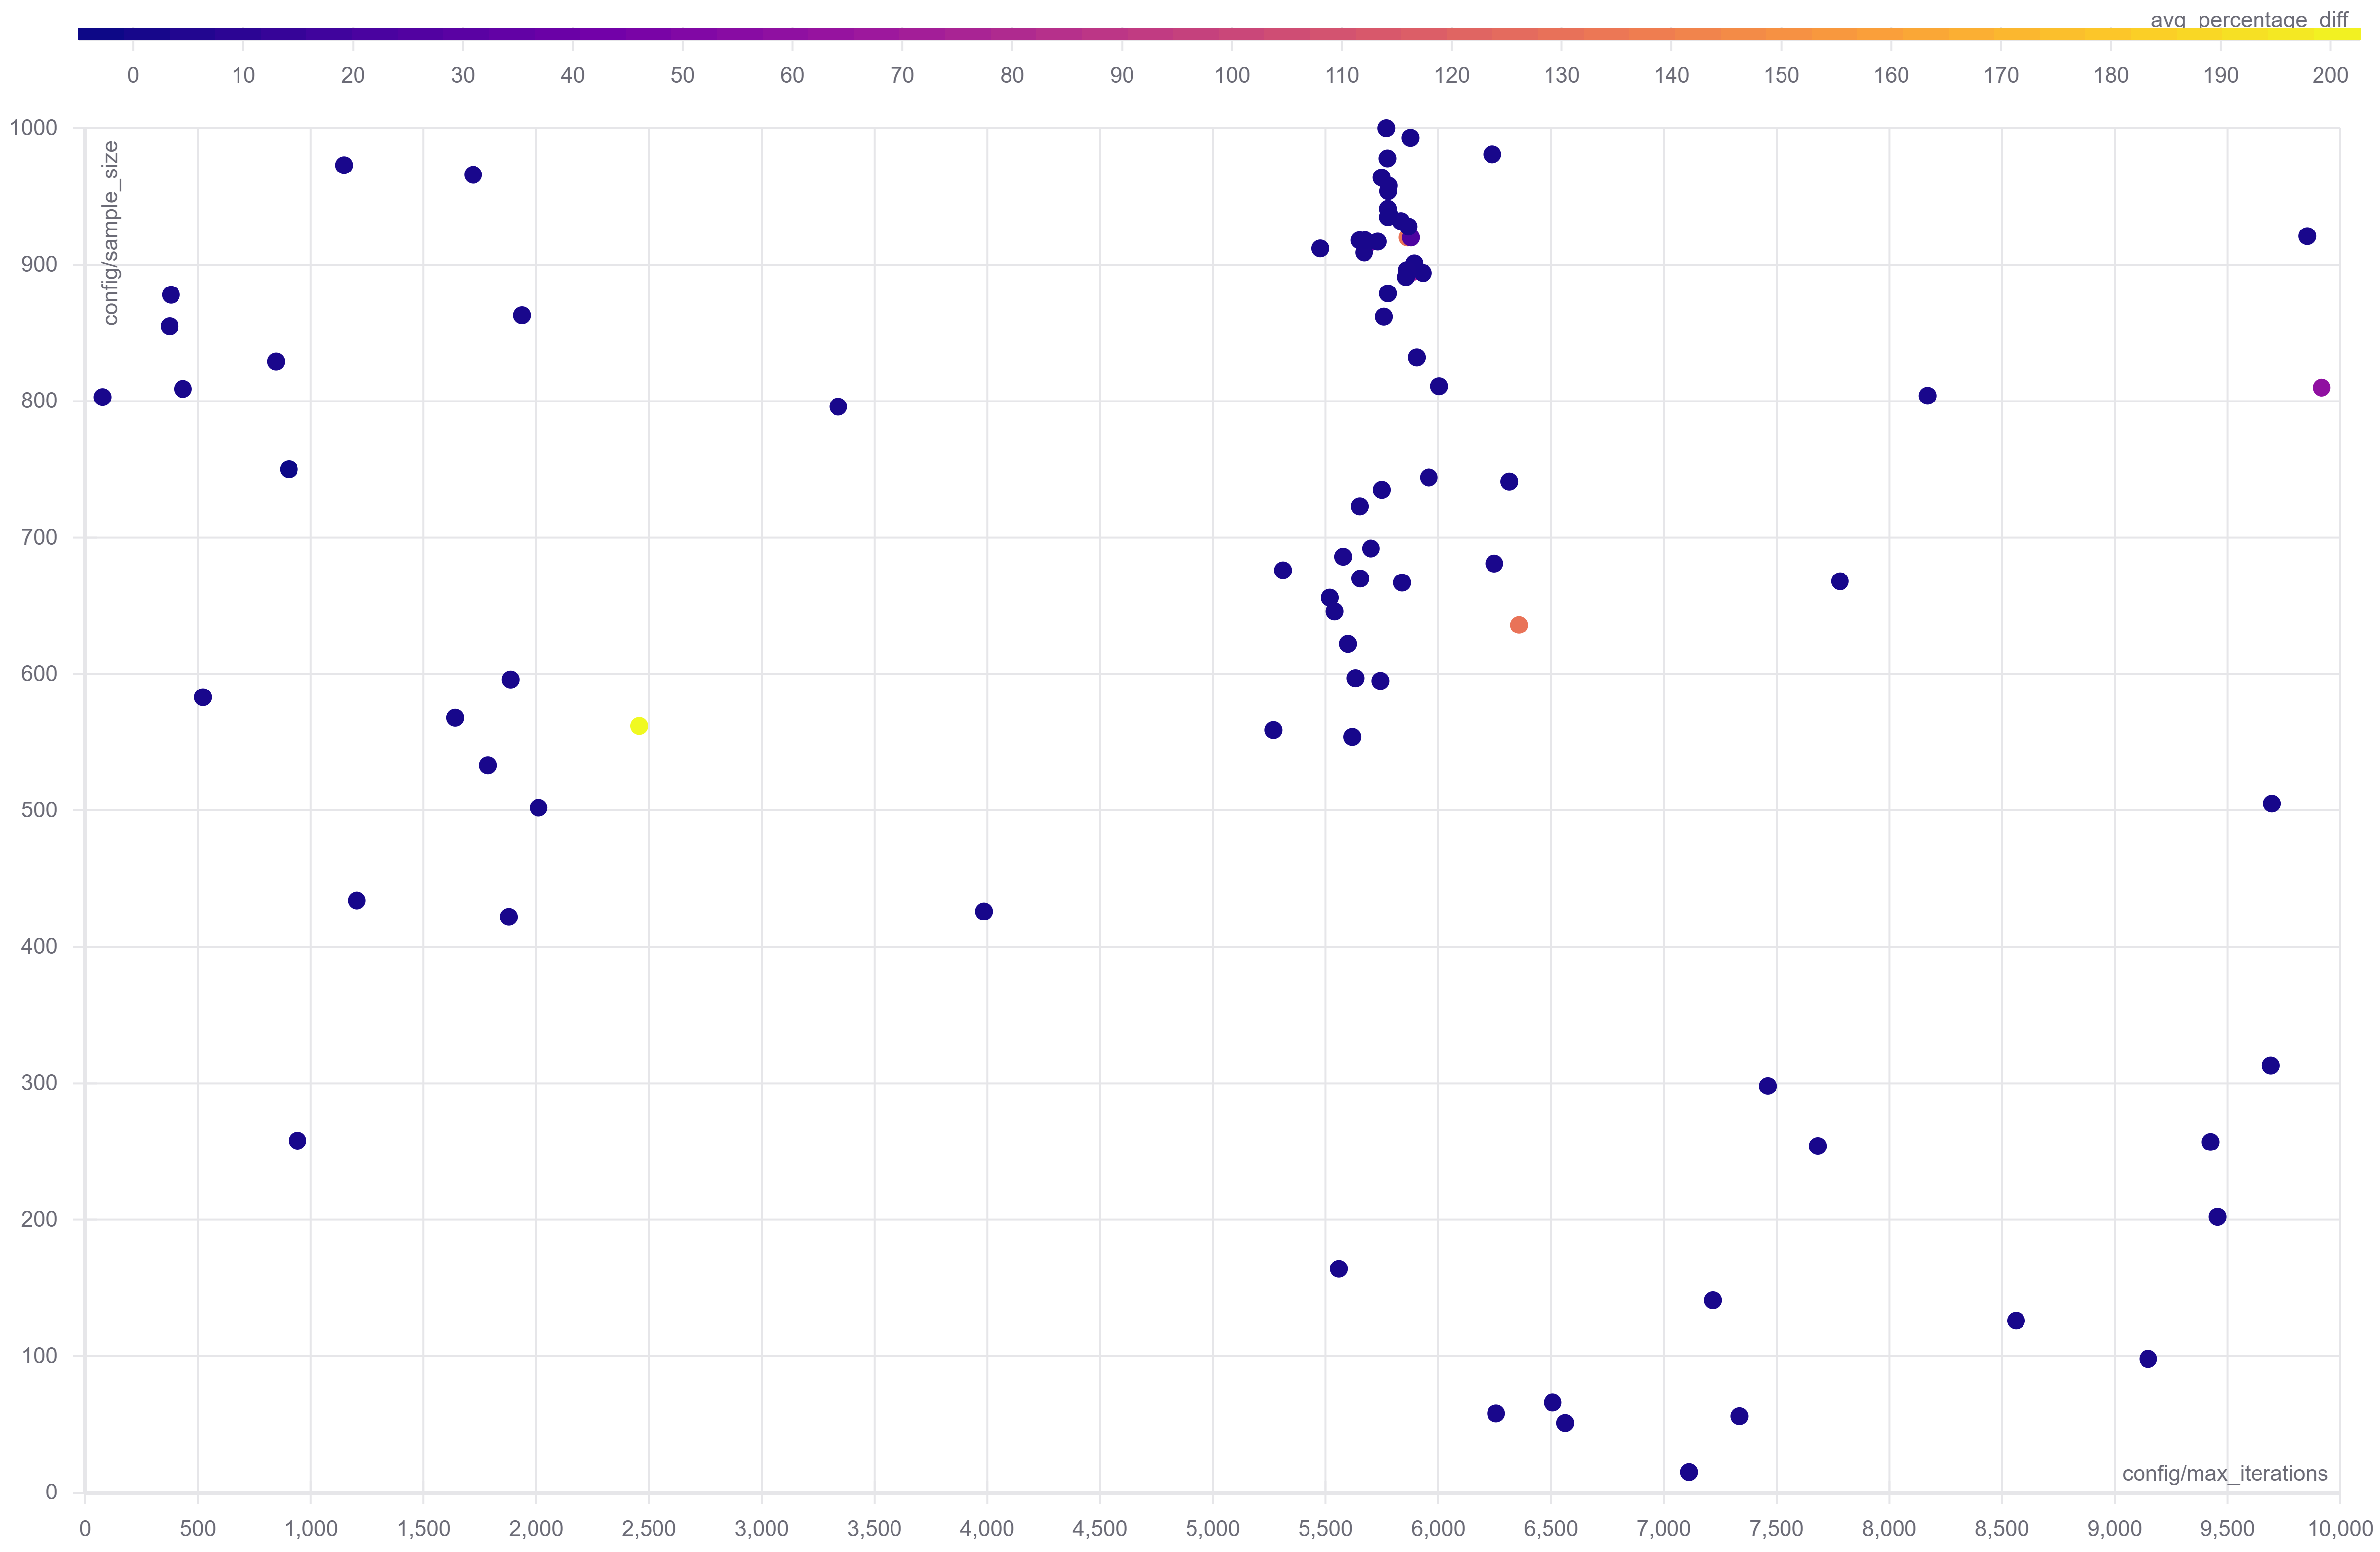
\includegraphics[width=\textwidth, keepaspectratio]{images/ss_mi_ad.png}
	\caption{Sample Size and Maximum Iterations v. Average Percentage Difference over default values}
	\label{fig:eval1}
	\end{figure}

	\item Best performing trials by percentage difference between obtained results over baseline values (figure \ref{fig:eval2}): this graph lets us see the best overall performing trials.

	\begin{figure}[h]
	\centering
	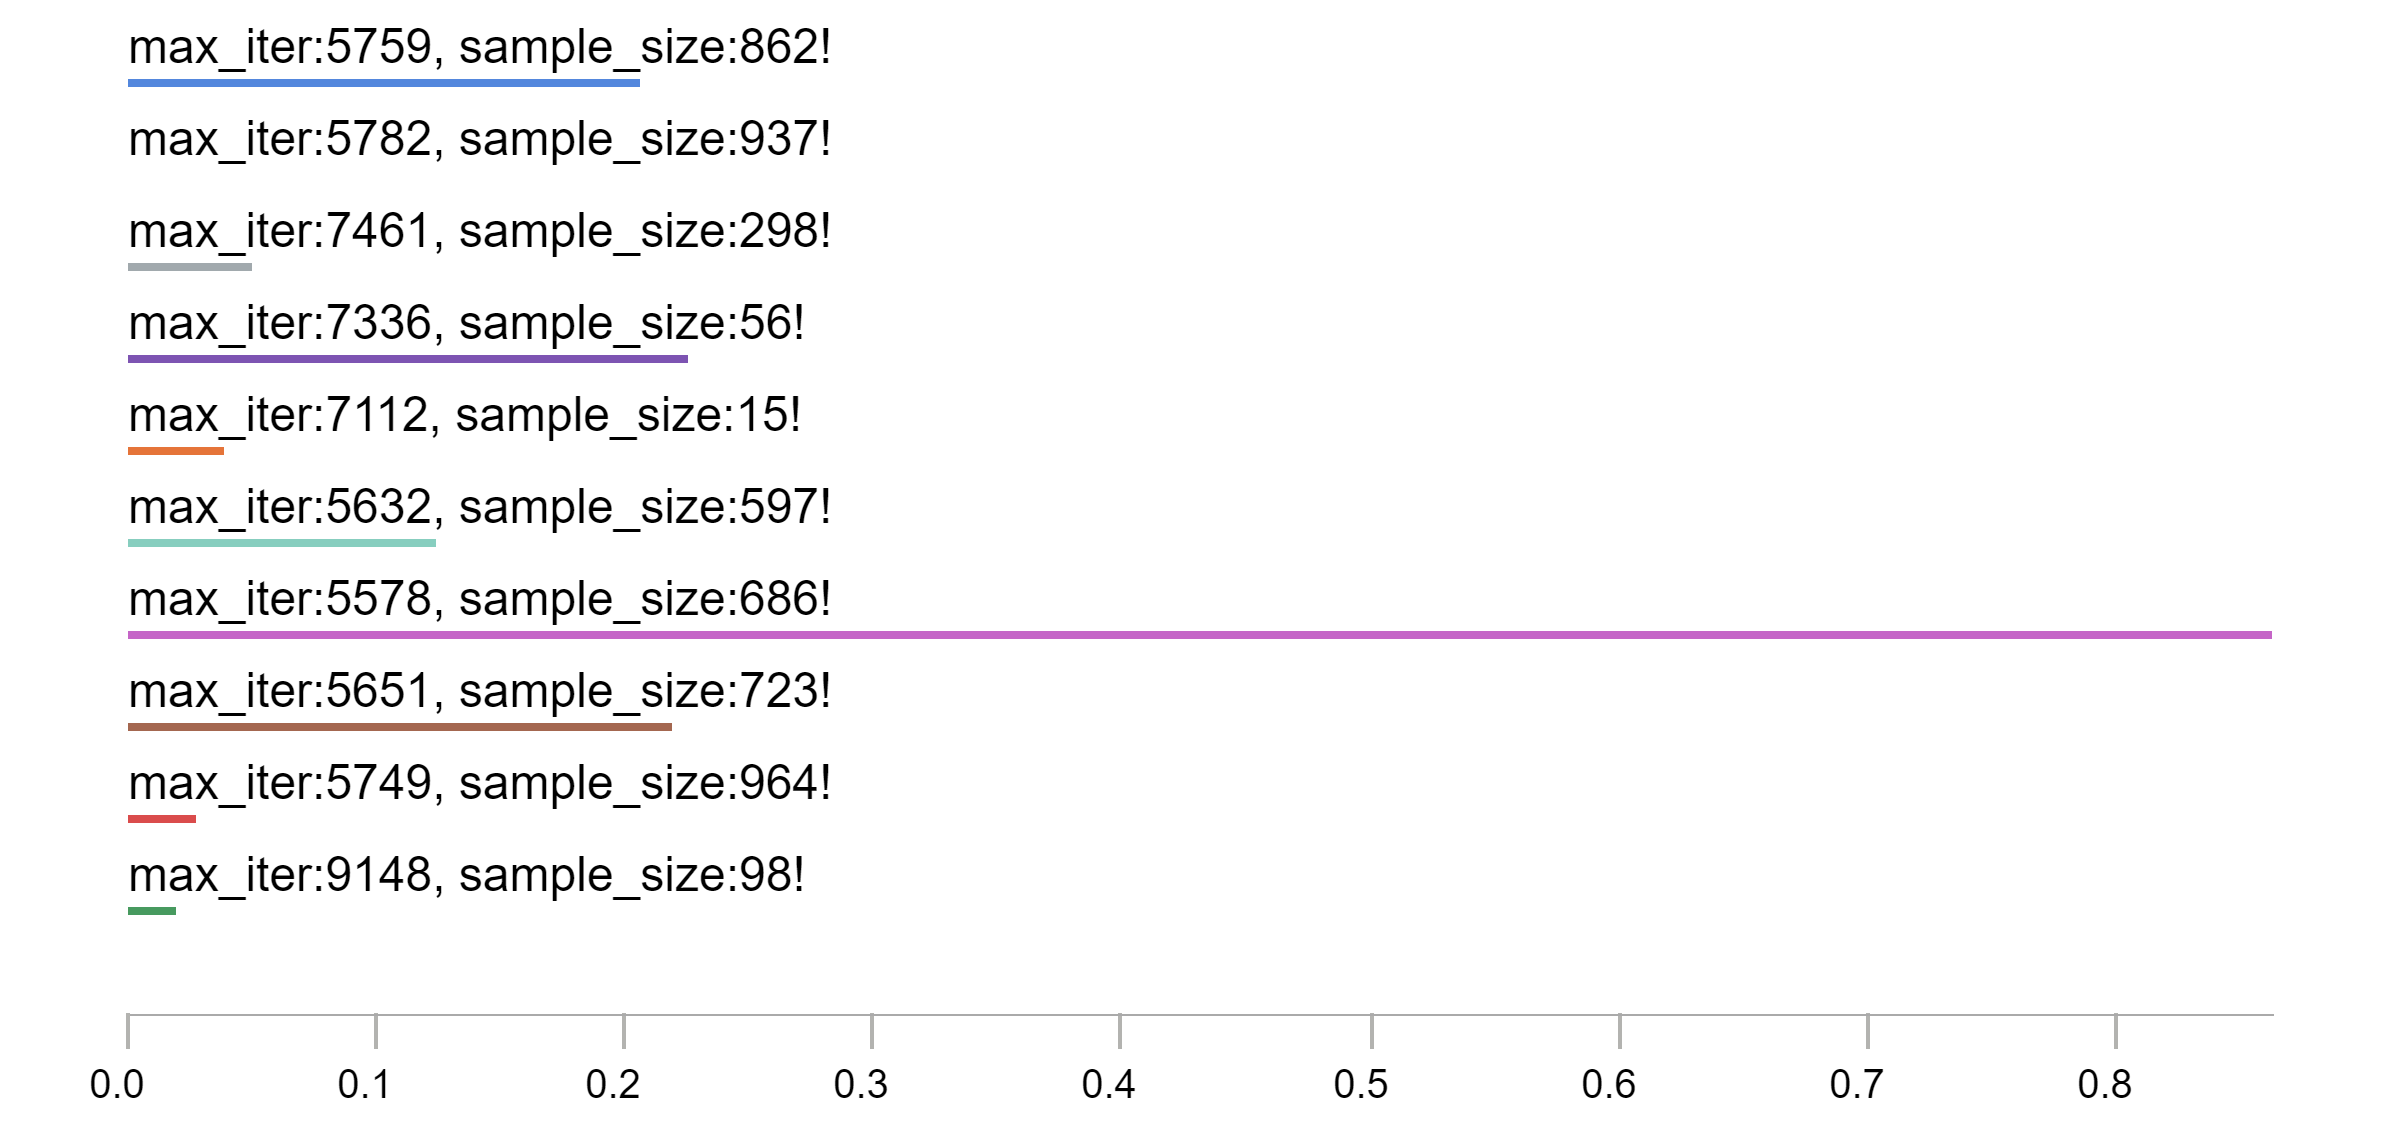
\includegraphics[width=\textwidth, keepaspectratio]{images/best_results.png}
	\caption{Best Percentage Differences over Baseline Values}
	\label{fig:eval2}
	\end{figure}

	\item Percentage difference between obtained results over baseline values, by training step (figure \ref{fig:eval3}): this graph lets us compare the performance of each trial for a any given point cloud.

	\begin{figure}[h]
	\centering
	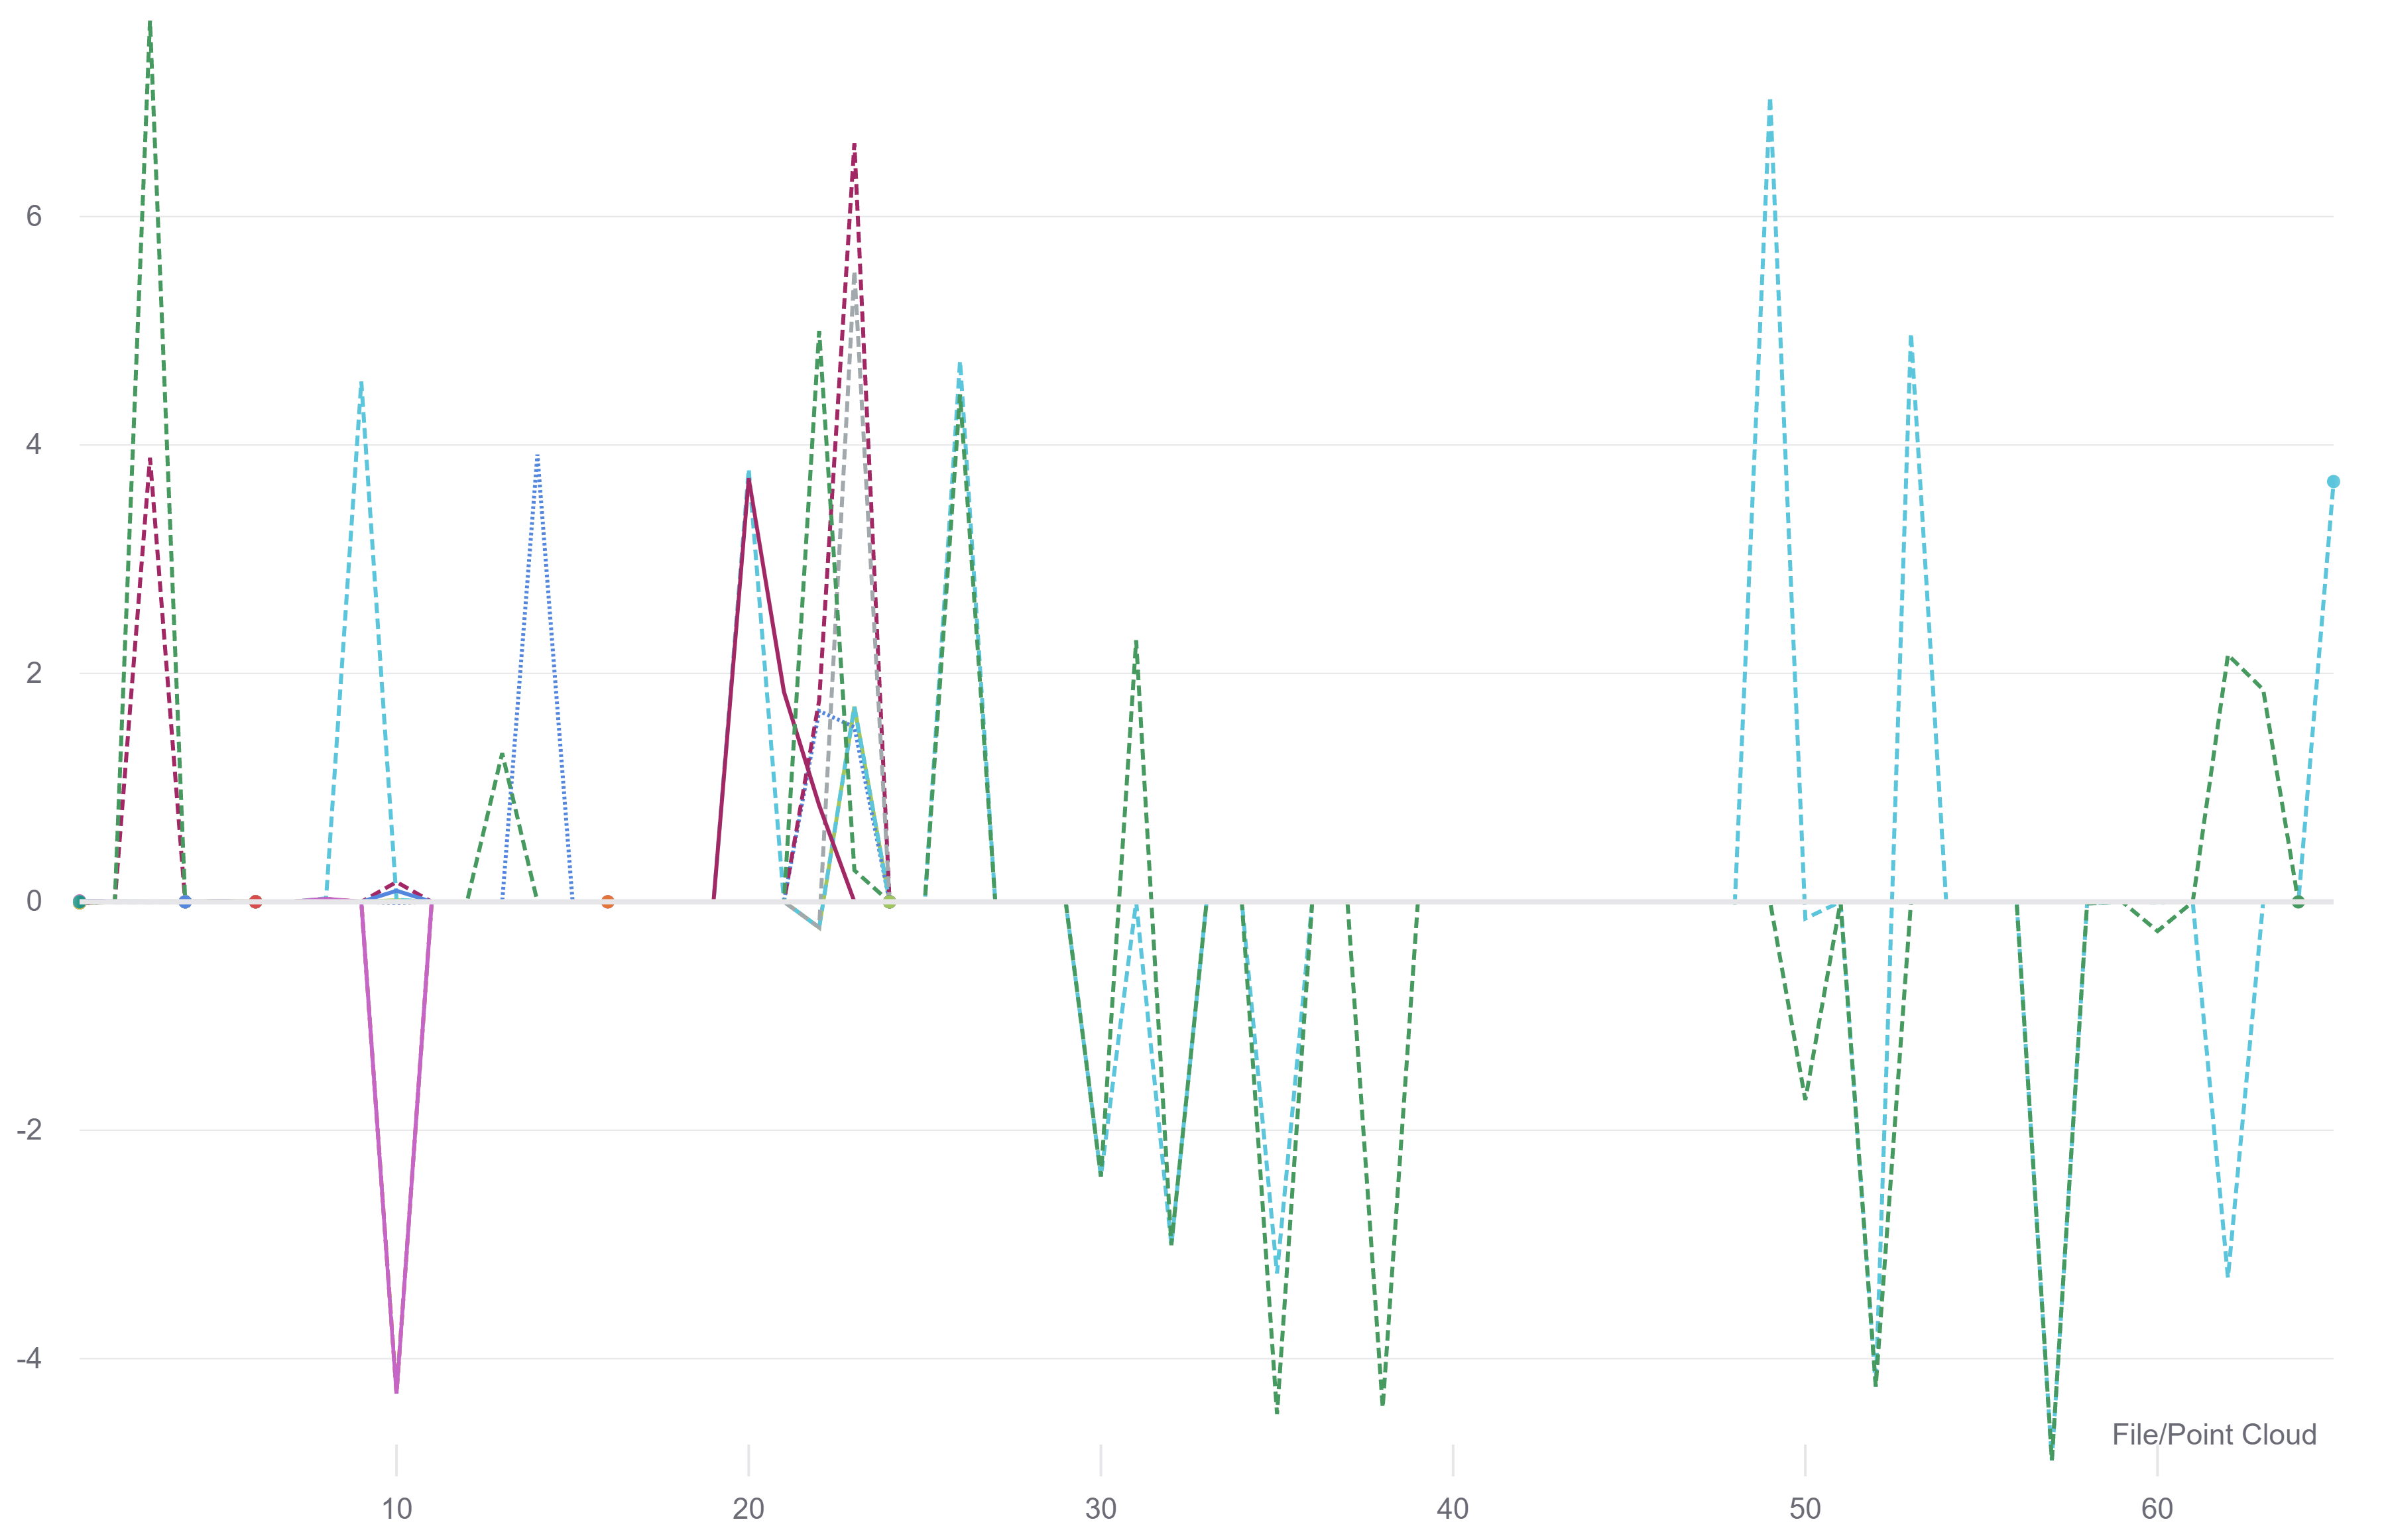
\includegraphics[width=\textwidth, keepaspectratio]{images/timeline.png}
	\caption{Percentage Difference over Baseline Values, by training iteration}
	\label{fig:eval3}
	\end{figure}

	\item Average Percentage difference between obtained results over baseline values, by training step (figure \ref{fig:eval4}): this graph lets us evaluate the evolution of the results over the training process.

	\begin{figure}[h]
	\centering
	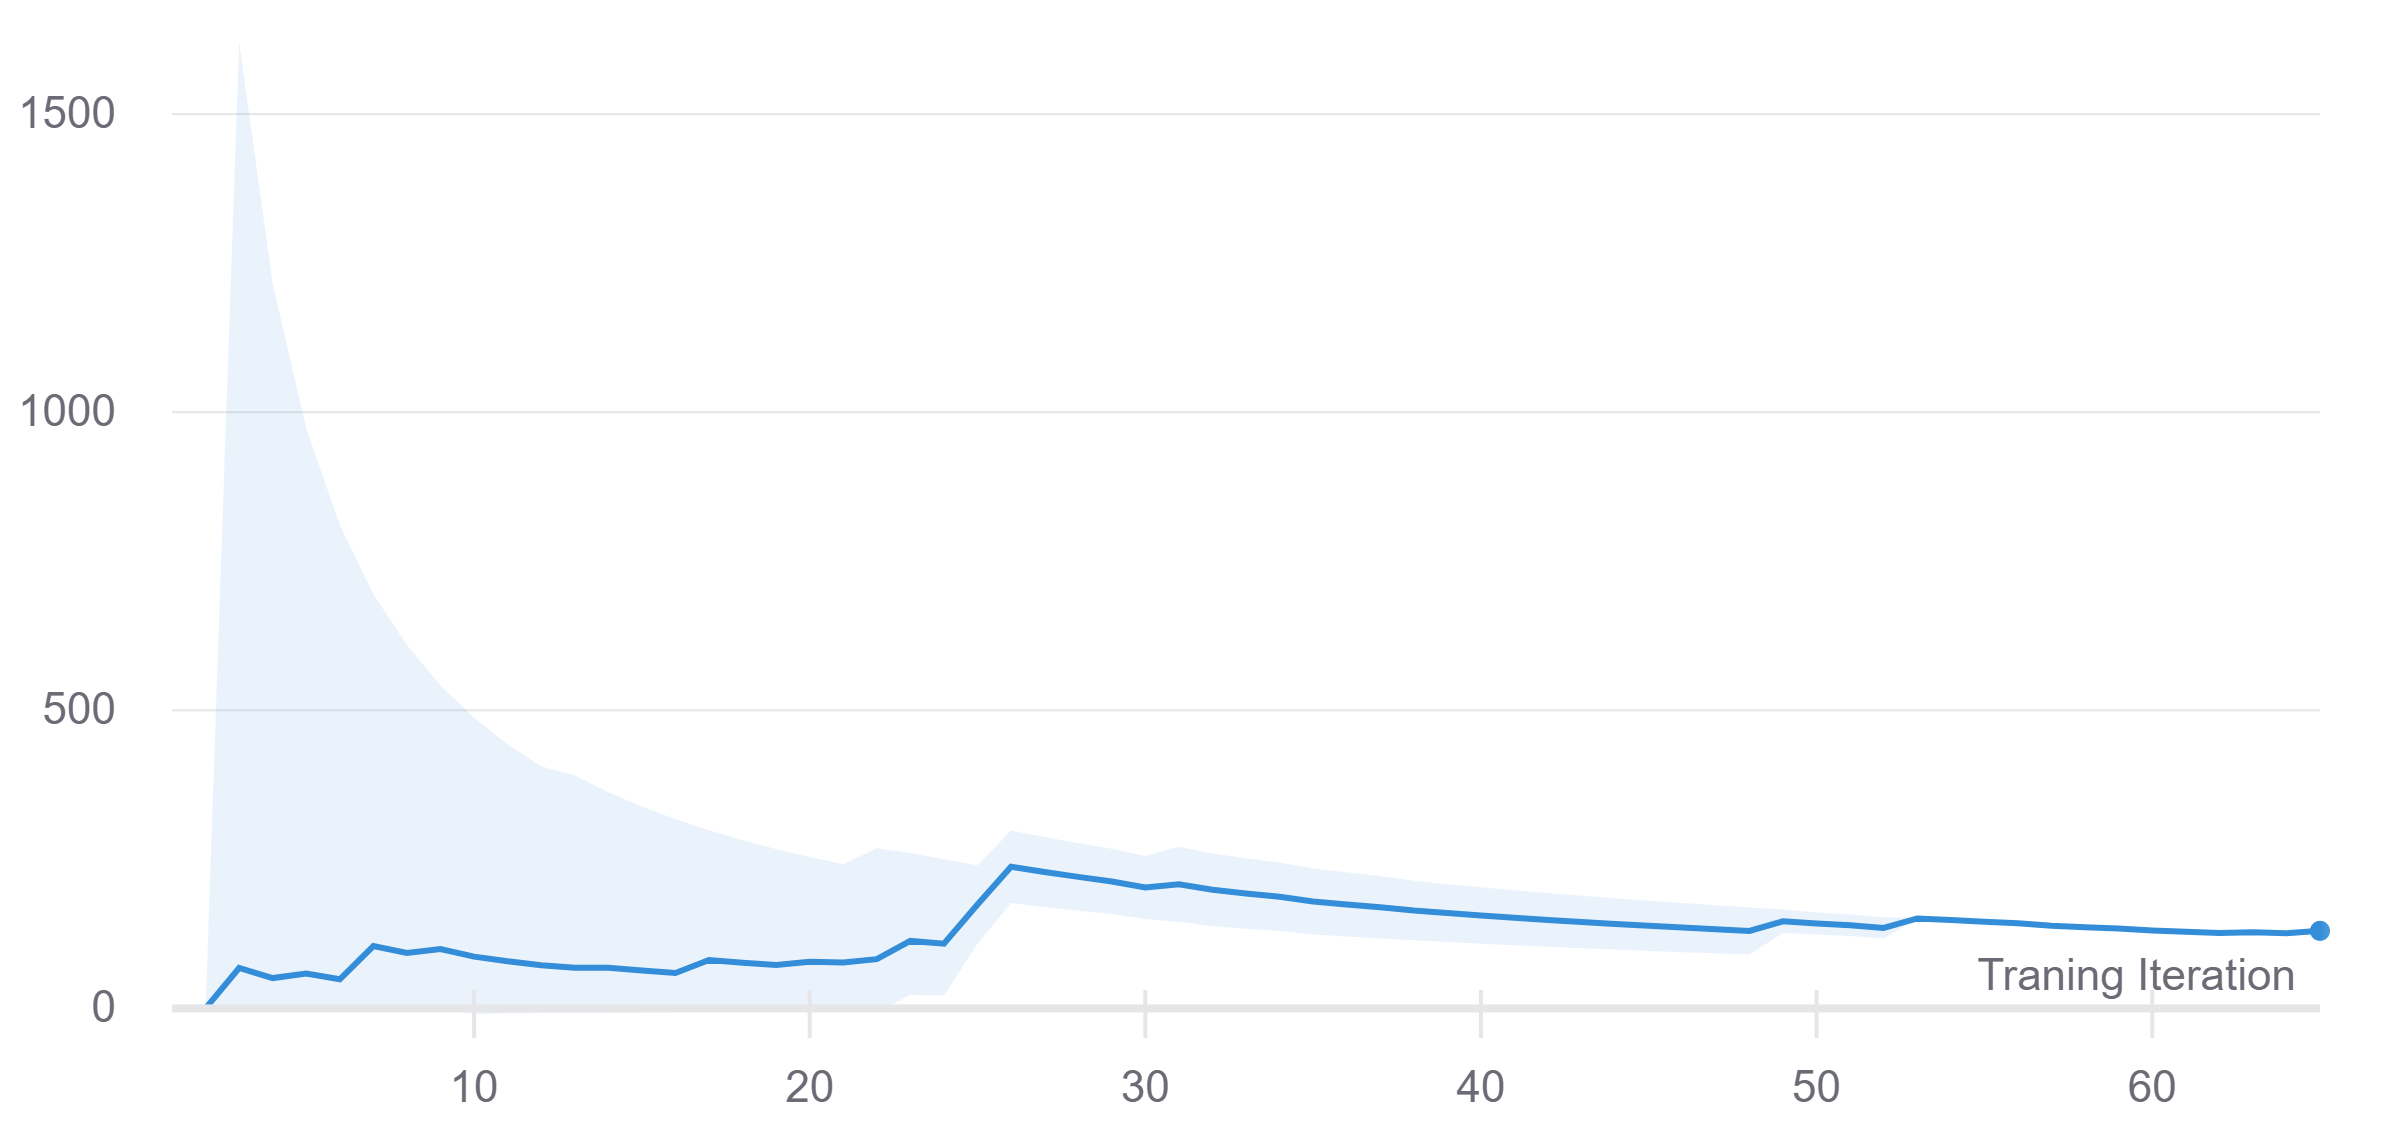
\includegraphics[width=\textwidth, keepaspectratio]{images/average_timeline.png}
	\caption{Average Percentage Difference over Baseline Values, by training iteration}
	\label{fig:eval4}
	\end{figure}

	\item Percentage difference between obtained results over baseline values, by training step, over time (figure \ref{fig:eval5}): this graph lets us evaluate the evolution of the results over the training process and over the actual \acrshort{hpo} execution time.

	\begin{figure}[h]
	\centering
	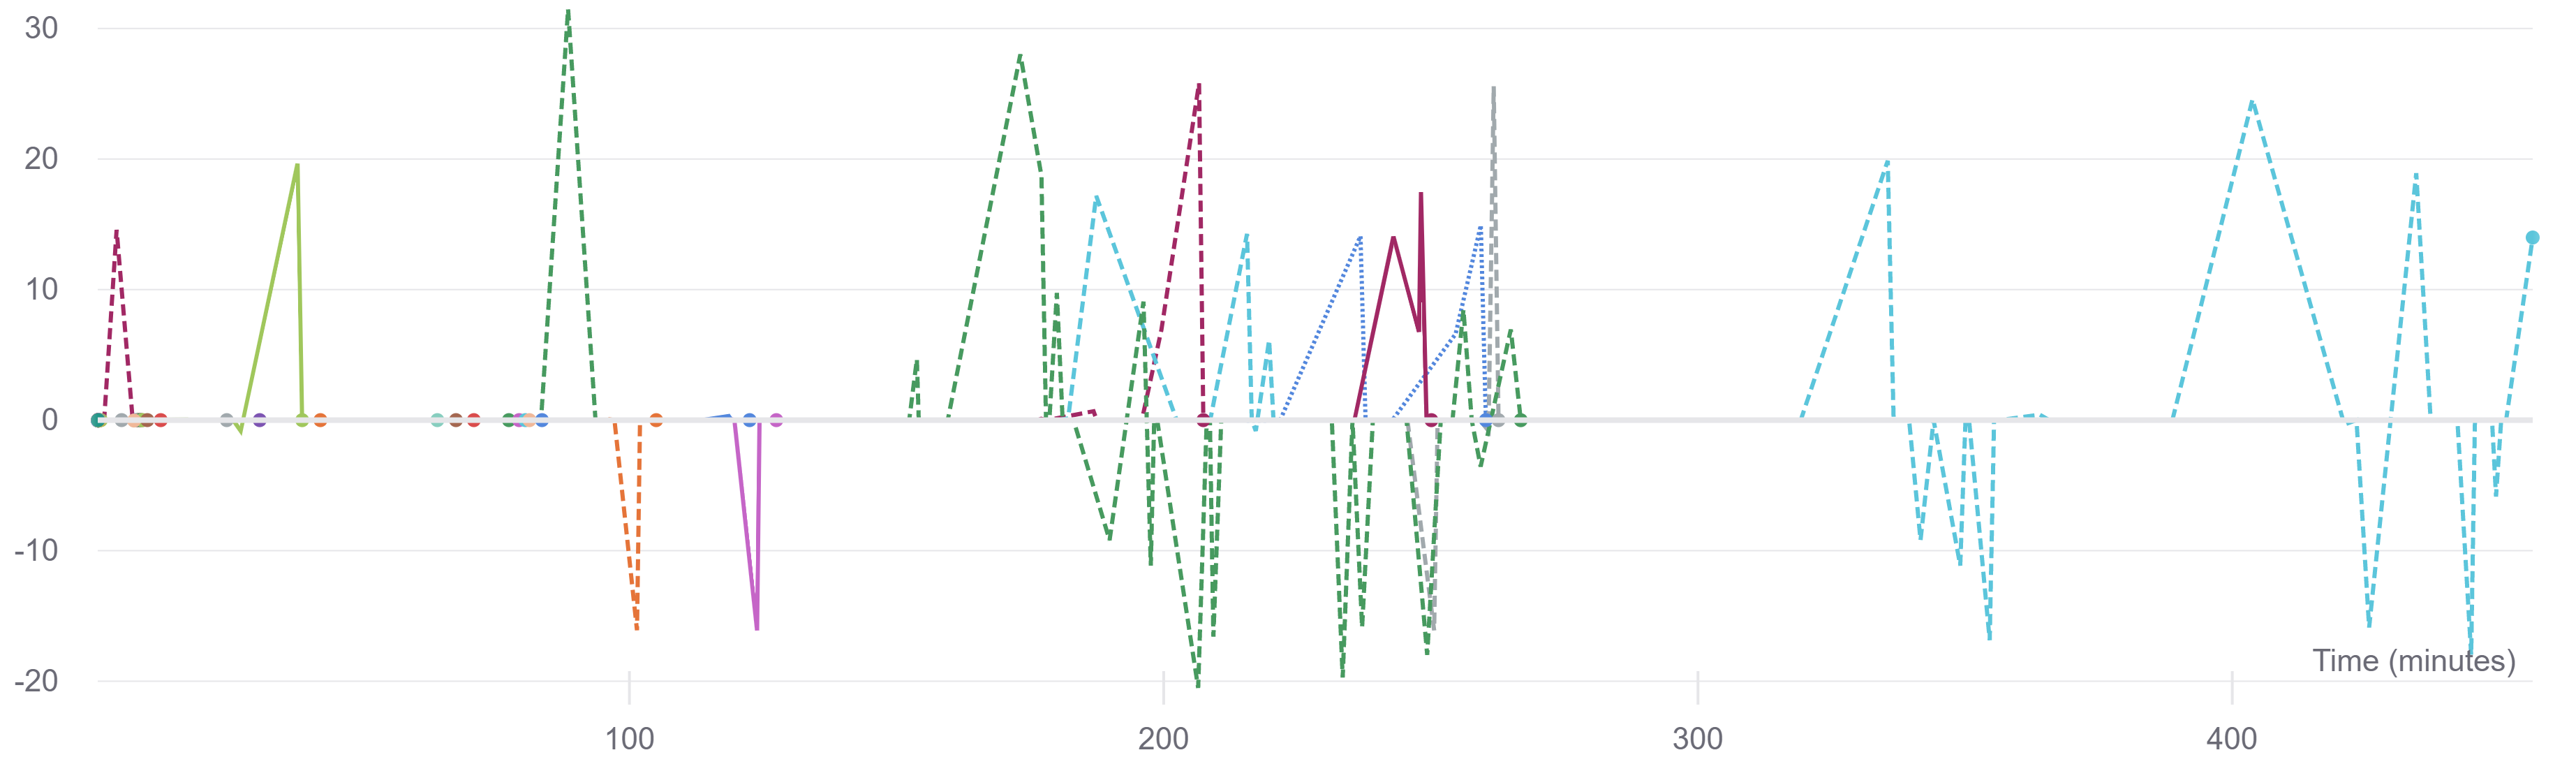
\includegraphics[width=\textwidth, keepaspectratio]{images/timed_timeline.png}
	\caption{Percentage Difference over Baseline Values, by training iteration, by wall time}
	\label{fig:eval5}
	\end{figure}

\end{itemize}

\subsubsection{Data Analysis}

From the obtained data and generated graphs we can draw some conclusions and gain some insights. These were also supplemented by information provided by the Research and Development team at \faro Portugal.

We can ascertain from analysing figure \ref{fig:eval1} that most hyper parameters value sets do not perform significantly better than the default hyper parameters. The best performing trials are found in the range between 500-700 for sample size, as well as in a narrower range between 5500-6500 for the max iterations.

We can also see that, overall, the best performing trials do not perform significantly better than the default hyper parameter values as even the best performing trial only has a $\approx 1\%$ improvement over the baseline value (see figure \ref{fig:eval2}).

These small improvements in previous observations are explained with figure \ref{fig:eval3}. In it, we can see that most for any given trial, most of the data points are close to the baseline values, while the best performing trials have a couple of outliers that skew the results. After further analysis, we have determined that this is a result of the data used and the sensitivity of the \acrshort{pca} algorithm to it. The point clouds that are being aligned range in size and complexity and the algorithm performance is very much dependant on the point cloud it is trying to align. Due to this we see better performance from in some point clouds over others, within each trial and for all trials as wells. We further develop this in the section \ref{sec:futurework}.

This issue is more evident in figure \ref{fig:eval4}, where we can see a peak of performance for one or two point clouds skews the data going forward, making it appear at is performing worse over time.

Finally, we can see in figure \ref{fig:eval5} that, even with the skewed results, the \acrshort{hpo} algorithm is performing well, culling bad performing trials early into the training process and using the obtained data to select new hyper parameter values, which are within the best performing trials overall. We also see that its attempt at optimizing the \acrshort{pca} function focuses on maximizing the results of a few point clouds, which skew the average percentage difference upward, fulfilling the goal of the algorithm.